%!TEX root = ../root.tex

\thispagestyle{empty}

\newgeometry{
left=3cm,
right=3cm,
top=2cm,
bottom=4cm
}

\begin{center}
\vspace*{1cm} \ \\
{\fontsize{40}{48}\selectfont \bfseries \mytitlewithlinebreaks \\}
\vspace{0.75cm}
{\Large\bfseries \mysubtitlewithlinebreaks \\}
\vspace{1.5cm}
\mytexttype \\
Studienjahrgang \myyearofstudy \\
Kurs \mycourse \\
\vspace{1.5cm}
Fakultät \myfaculty \\
Studiengang \mycourseofstudy \\
DUALE HOCHSCHULE BADEN-WÜRTTEMBERG\\
VILLINGEN-SCHWENNINGEN\\
\end{center}
\begin{textblock*}{50mm}(40mm,180mm)
    \begin{rotate}{50}
        \fontsize{34}{40}\bfseries\textcolor{red}{Sperrvermerk}
    \end{rotate}
\end{textblock*}
\begin{table}[b]
\begin{tabular}{ll}
Bearbeiter: 		&	\myauthor \\
Ausbildungsbetrieb:	&	\mycompany \\
Betreuender Dozent:	&	\mylecturer \\
\end{tabular}\\
\\
\\
\begin{tabularx}{\textwidth}{lXl}

\includegraphics[width=.3\linewidth]{title/dhbw-vs-logo} &
&
\raisebox{\height}{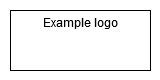
\includegraphics[width=.3\linewidth]{title/company-logo} }
\end{tabularx}
\end{table}

\restoregeometry
